\documentclass[letterpaper,12pt]{book}
\usepackage[margin=0.75in]{geometry}
% Wait to usepackage these until they are needed.
% \usepackage{moreverb}
% \usepackage{float}
% \usepackage{subfigure}
\usepackage{graphicx}
\usepackage{wrapfig}
\usepackage{color}
% \usepackage{epstopdf}

% Again, uncomment when/if needed.
% % Define the \sourcelst command to create a floating listing of 
% % a (separate) source file.
% \newfloat{listing}{t}{lop}
% \floatname{listing}{Listing}
% \def\sourcelst#1#2{
% \begin{listing}
% \begin{tabular}{|@{\hspace{0.04\linewidth}}c@{\hspace{0.02\linewidth}}|}
% \hline \\
% \begin{minipage}{0.94\linewidth}
% \small\listinginput{1}{#1}
% \end{minipage}
% \\ \\ \hline
% \end{tabular}
% \caption{[{\tt #1}]\ \ #2}
% \label{lst:#1}
% \end{listing}
% }

\title{{\Huge The Ames Stereo Pipeline:}\\A User's Guide to the\\NASA Ames Stereo Pipeline v1.0 ALPHA}
\author{
Michael J.~Broxton\\
Ross A.~Beyer\\
Zachary Moratto\\
Mike Lundy\\
\\
Intelligent Systems Division\\
NASA Ames Research Center\\
\\
DRAFT}

\begin{document}
\maketitle

\chapter*{Credits}

This open source version of the Ames Stereo Pipeline (ASP) was
developed by the Intelligent Robotics Group (IRG), in the Intelligent
Systems Division at NASA Ames Research Center in Moffett Field, CA. It
builds on over ten years of IRG experience developing surface
reconstruction tools for terrestrial robotic field tests and planetary
exploration. \\

{\bf Principal Investigator, NASA Ames Planetary Mapping and Modeling Team}
\begin {itemize} 
\item Michael J.~Broxton (NASA/Carnegie Mellon University)\\ {\tt
  michael.broxton@nasa.gov}\\
\end{itemize}

{\bf Lead Developer \& Stereo Pipeline Project Lead}
\begin {itemize} 
\item Zachary Moratto (NASA/Stinger-Ghaffarian Technologies)
\end{itemize}

{\bf Development Team}
\begin{itemize}
\item Dr.~Ross Beyer (NASA/SETI Institute)
\item Dr.~Ara Nefian (NASA/Carnegie Mellon University)
\item Matthew Hancher (NASA)
\item Kyle Husmann (NASA/Educational Associates Program)
\item Mike Lundy (NASA/Stinger-Ghaffarian Technologies)
\item Vinh To (NASA/Stinger-Ghaffarian Technologies)
\end{itemize}

{\bf Contributing Developer \& Former IRG Terrain Reconstruction Lead:}
\begin{itemize}
\item Dr.\ Laurence Edwards (NASA)
\end{itemize}

A number of student interns have made significant contributions to
this project over the years: Sasha Aravkin (Washington State
University), Kyle Hussman (California Polytechnic Institute), Patrick
Mihelich (Stanford University), Melissa Bunte (Arizona State
University), Matthew Faulkner (Massachusetts Institute of Technology),
Todd Templeton (UC Berkeley), Morgon Kanter (Bard College), Kerri
Cahoy (Stanford University), and Ian Saxton (UC San Diego).

The open source stereo pipeline leverages stereo image processing
work, past and present, led by Dr. Laurence Edwards, Eric Zbinden
(formerly NASA/QSS Inc.), Dr.~Michael Sims (NASA), and others in the
Intelligent Systems Division at NASA Ames Research Center. It has
benefited substantially from the contributions of Dr.~Keith Nishihara
(formerly NASA/Stanford), Randy Sargent (NASA/Carnegie Mellon
University), Dr.~Judd Bowman (formerly NASA/QSS Inc.), Clay Kunz
(formerly NASA/QSS Inc.), and Dr.~Matthew Deans (NASA).

\section*{Acknowledgements}

The initial adaptation of Ames' stereo surface reconstruction tools to
orbital imagers was a result of a NASA funded, industry led project to
develop automated Digital Elevation Model generation techniques for
the Mars Global Surveyor (MGS) mission. Our work with the project's
Principle Investigator, Dr.~Michael Malin of Malin Space Science
Systems (MSSS), and Co-Investigator, Dr.~Laurence Edwards of NASA
Ames, inspired the idea of making stereo surface reconstruction
technology available and accessible to a broader community.  We thank
Dr.~Malin and Dr.~Edwards for providing the initial impetus that in no
small way made this open source stereo pipeline possible, and we thank
Dr.~Michael Caplinger, Joe Fahle and others at MSSS for their help and
technical assistance.

We'd also like to thank our friends and collaborators Dr.~Randolph
Kirk, Dr.~Brent Archinal, Trent Hare, and Dr.~Mark Rosiek of the USGS
Astrogeology Branch in Flagstaff, AZ for their encouragement and
willingness to share their experience and expertise by answering many
of our technical questions.  We also thank them for their ongoing
support and efforts to help us evaluate our work.  Thanks also to the
USGS ISIS team, especially Jeff Anderson and Kris Becker, for their
help in integrating this version of the stereo pipeline with the USGS
ISIS software package.

Thanks go also to Dr.~Mark Robinson, Jacob Danton, Ernest
Bowman-Cisneros, Dr.~Sam Laurence, and Melissa Bunte at Arizona State
University for their help in adapting the Ames' stereo pipeline to
lunar data sets including the Apollo Metric Camera.

Finally, we thank Melissa Bunte, Dr.~Ara Nefian, and Dr.~Laurence
Edwards for their contributions to this documentation, and Dr.~Terry
Fong (IRG Group Lead) for his management and support of the open
source \& public software release process.

Portions of this software were developed with support from the
following NASA funding sources: the Mars Technology Program, the Mars
Critical Data Products Initiative, the Mars Reconnaissance Orbiter
mission, the Applied Information Systems Research program grant
\#06-AISRP06-0142, the Lunar Advanced Science and Exploration Research
(LASER) program grant \#07-LASER07-0148, and the ESMD Lunar Mapping and
Modeling Program (LMMP).

\tableofcontents
\chapter{Introduction}

The NASA Ames Stereo Pipeline (ASP) is a suite of automated geodesy \&
stereogrammetry tools designed for processing planetary imagery
captured from orbiting and landed robotic explorers on other planets.
It was designed to process stereo imagery captured by NASA spacecraft
and produce cartographic products including digital elevation models
(DEMs), ortho-projected imagery, and 3D models.  These data products
are suitable for science analysis, mission planning, and public
outreach.

\begin{figure}[tb] 
   \centering
   \includegraphics[width=6.5in]{images/introduction/p19view2.png} 
   \caption{This 3D model was generated from Mars Orbiter Camra image
     pair M01-00115 and E02-01461 (34.66N, 141.29E).  The complete
     stereo reconstruction process takes approximately five minutes on
     a 3.0GHz workstation for input images of this size (1024x8064
     pixels).  This model, shown here without vertical elevation
     exaggeration, is roughly 2-km wide in the cross-track
     dimension. }
   \label{fig:p19}
\end{figure}

\section{Background}

The Intelligent Robotics Group (IRG) at the NASA Ames Research Center
has been developing 3D surface reconstruction and visualization
capabilities for planetary exploration for more than a decade.  First
demonstrated during the Mars Pathfinder Mission, the IRG has delivered
tools providing these capabilities to the science operations teams of
the Mars Polar Lander mission, the Mars Exploration Rover mission, and
most recently the Mars Reconaissance Orbiter Mission. A critical
component technology enabling this work is the Ames Stereo Pipeline.
ASP generates high quality, dense, texture-mapped 3D surface models
from stereo image pairs.

Although initially developed for ground control and scientific
visualization applications, the ASP has evolved in recent years to
address orbital stereogrammetry and cartographic applications.  In
particular, long-range mission planning requires detailed knowledge of
planetary topography, and high resolution topography is often derived
from stereo pairs captured from orbit.  Orbital mapping satellites are
sent as precursors to planetary bodies in advance of landers and
rovers.  They return a wealth of imagery and other data that helps
mission planners and scientist identify areas worthy of more detailed
study. Topographic information often plays a central role in this
planning and analysis process.

Laser range-finding instruments such as the Mars Orbital Laser
Altimeter (MOLA) \citep{1992JGR....97.7781Z,2001JGR...10623689S}
has significantly advanced the study of the Martian surface by
providing geologists with a highly accurate elevation map of the
entire planet.  The upcoming Lunar Orbital Laser Altimeter (LOLA)
\citep{2008AGUFM.P31B1419N,2007SSRv..129..391C} will achieve similar
results for the Moon.  However, MOLA topographic products are limited
in resolution (463~m/pixel at the equator).  This, coupled with
localized interpolation artifacts in some regions due to sparse
laser data, have rendered MOLA products insufficient for detailed
studies of specific sites; e.g. geologic stratification and deposition
analysis, or in the case of mission planning, landing site selection.

The most common technique for obtaining higher-resolution digital
terrain models (DTMs) is to employ stereogrammetric techniques.
However, existing processing techniques on photogrammetric
workstations are extremely human intensive and expensive.  The
substantial number of man-hours and resources required for this
approach has meant that relatively few of the existing stereo image
pairs have been processed, hence very few of these data products have
reached the scientific community.

The ASP was designed to address this shortfall by automating the
stereo reconstruction process so that it can run without human
guidance.  By applying recent advances in robotics and computer
vision, we have created an automated process that is capable of
generating high quality DEMs with minimal human intervention.  Users
of the Stereo Pipeline can expect to spend some time picking a handful
of settings when they first start processing a new type of imagery,
but once this is done the Stereo Pipeline can be used to process tens,
hundreds, or even thousands of stereo pairs without further
adjustment.


\section{Operation with the USGS Integrated Software for Imagers and Spectrometers}

This version of the Stereo Pipeline functions as an add-on for an
existing installation of the USGS Integrated Software for Imagers and
Spectrometers (ISIS).  ISIS is widely used in the planetary science
community for processing raw spacecraft imagery into high level data
products of scientific interest such as map projected and mosaicked
imagery \cite{2004LPI....35.2039A, 1997LPI....28..387G, ISIS_website}.

The Stereo Pipeline provides an advanced stereo image processing
capability for ISIS.  It supports the ISIS ``cube'' file format, and
can make use of the ISIS camera models and ancillary information
(i.e. SPICE kernels) for imagers on many NASA spacecraft.  This tight
integration with ISIS allows scientists to prepare data and perform
stereo processing using the familiar ISIS toolchain.  Another benefit
is that new sensor models are available in the ASP as soon as they are
developed for ISIS.  In principal, by leveraging the wealth of
different camera models in ISIS, stereo processing can even be carried
out with images captured by different spacecraft.  Finally, and
perhaps most importantly, the use of a single standardized set of
camera models also ensures consistency between products generated in
the Stereo Pipeline and those generated by ISIS.

The Stereo Pipeline can process arbitrary, non-ISIS images with
accompanying camera information, but doing so requires a significant
amount of extra work and setup.  This use is not covered in this
document, however feel free to contact us if you are interested in
learning more about the software's advanced capabilities.

\section{Terminology}

DISPARTY

TRIANGULATION

CORRELATION

BUNDLE ADQJUSTMENT

\section{Getting Help}

All bugs, feature requests, and general discussion should be sent to
the Ames Stereo Pipeline user mailing list:
\begin{quote}
\indent \url{stereo-pipeline@lists.nasa.gov}
\end{quote}
To subscribe to this list, send an empty email message with the
subject 'subscribe' (without the quotes) to:
\begin{quote}
\indent \url{stereo-pipeline-request.lists.nasa.gov}
\end{quote}
To contact the lead developers and project manager directly, send mail
to:
\begin{quote}
\indent \url{stereo-pipeline-owner@lists.nasa.gov}
\end{quote}

\section{Warnings to users of the Ames Stereo Pipeline ALPHA}

This is an {\bf ALPHA} release of the Stereo Pipeline.  There are many
known bugs and incomplete features. The API and command line options
will almost certainly change prior to the final release.  Some of the
documentation is incomplete and some of it may be out of date or
incorrect.  Although we hope you will find this release helpful, you
use it at your own risk.

While we are confident that the algorithms used by this software are
robust, they have not been systematically tested or rigorously
compared to other methods in the peer-reviewed literature. We have a
number of efforts underway to carefully compare Stereo
Pipeline-generated data products to those produced by established
processes, and we will publish those results as they become available.
In the meantime, {\bf we strongly recommend that you consult us before
  publishing any results based on the cartographic products produced
  by this software}. You have been warned!




\chapter{Installation}

\section{Binary Installation}

This is the recommended method. Only the Stereo Pipeline binaries
are required. ISIS is required only for users who wish to process
NASA non-terrestrial imagery.  A full ISIS installation is not
required for operation of Stereo Pipeline programs (only the ISIS
data directory is needed), but is required for certain preprocessing
steps before Stereo Pipeline programs are run for planetary data.
If you only want to process terrestrial Digital Globe imagery, skip
to section \ref{quickstartDG}.

\begin{description}
\item [{Stereo~Pipeline~Tarball}] \hspace*{\fill} \\
The main Stereo Pipeline page is
\url{http://irg.arc.nasa.gov/ngt/stereo}.  Download the option that
matches the platform you wish to use. The recommended, but
optional, \ac{ISIS} version is listed next to the name.

\item [{USGS~ISIS}] \hspace*{\fill} \\
If you are working with non-terrestrial imagery, you will need to install
\ac{ISIS} so that you can perform preprocessing such as radiometric
calibration and ephemeris attachment. The \ac{ISIS} installation guide is at
\url{http://isis.astrogeology.usgs.gov/documents/InstallGuide}.  You
must use their binaries as-is; if you need to recompile, you can
follow the \emph{Source Installation} guide for the Stereo Pipeline in
Section~\ref{sec:Source-Installation}.  Note also that the \ac{USGS}
provides only the current version of \ac{ISIS} and the previous
version (denoted with a `\texttt{\_OLD}' suffix) via their
\texttt{rsync} service. If the current version is newer than the
version of ISIS that the Stereo Pipeline is compiled against, be
assured that we're working on rolling out a new version. However,
since Stereo Pipeline has its own self-contained version of ISIS's
libraries built internally, you should be able to use a newer version
of ISIS with the now dated version of \ac{ASP}. This is assuming no major
changes have taken place in the data formats or camera models by
\ac{USGS}. At the very least, you should be able to rsync the previous
version of ISIS if a break is found.  To do so, view the listing of
modules that is provided via the
`\texttt{rsync~isisdist.astrogeology.usgs.gov::}' command.  You should
see several modules listed with the `\texttt{\_OLD}' suffix.  Select
the one that is appropriate for your system, and \texttt{rsync}
according to the instructions.

In closing, running the Stereo Pipeline executables only requires that
you have downloaded the ISIS secondary data and have appropriately set
the \texttt{ISIS3DATA} environment variable. This is normally
performed for the user by ISIS startup script,
\texttt{\$ISISROOT/scripts/isis3Startup.sh}.

\end{description}

\subsection{Quick Start for ISIS Users}
\begin{description}

\item[{Fetch~Stereo~Pipeline}] ~\\
Download the Stereo Pipeline from \url{http://irg.arc.nasa.gov/ngt/stereo}.

\item [{Fetch~ISIS~Binaries}] ~\\
As detailed at \url{http://isis.astrogeology.usgs.gov/documents/InstallGuide}.

\item [{Fetch~ISIS~Data}] ~\\
As detailed at \url{http://isis.astrogeology.usgs.gov/documents/InstallGuide}.

\item [{Untar~Stereo~Pipeline}] ~\\
\texttt{tar xzvf StereoPipeline-\textit{VERSION-ARCH-OS}.tar.gz}

% Verbatim has way too much white space. Couldn't seem to take care of it with
% vskip/vspace negative. Sigh.
\item [{Add~Stereo~Pipeline~to~Path~(optional)}] ~\\
bash: \texttt{export PATH="\textit{/path/to/StereoPipeline}/bin:\$\{PATH\}"} \\
csh:  \texttt{setenv PATH "\textit{/path/to/StereoPipeline}/bin:\$\{PATH\}"}

\item[Set~Up~ISIS] ~\\
bash: \\
\hspace*{2em}\texttt{export ISISROOT=\textit{/path/to/isisroot}} \\
\hspace*{2em}\texttt{source \$ISISROOT/scripts/isis3Startup.sh} \\
csh: \\
\hspace*{2em}\texttt{setenv ISISROOT \textit{/path/to/isisroot}} \\
\hspace*{2em}\texttt{source \$ISISROOT/scripts/isis3Startup.csh}

\item [{Try~It~Out}] ~\\
See Chapter~\ref{ch:moc_tutorial} for an example.
\end{description}

\subsection{Quick Start for Digital Globe Users}
\label{quickstartDG}
\begin{description}

\item[{Fetch~Stereo~Pipeline}] ~\\
Download the Stereo Pipeline from \url{http://irg.arc.nasa.gov/ngt/stereo}.

\item[{Untar~Stereo~Pipeline}] ~\\
\texttt{tar xvfz StereoPipeline-\textit{VERSION-ARCH-OS}.tar.gz}

\item [{Try~It~Out}] ~\\
Processing Earth imagery is described in the data processing tutorial
in chapter \ref{ch:dg_tutorial}.

\end{description}

\subsection{Quick Start for Aerial and Historical Imagery}
\label{quickstartAerial}

Fetch the software as before. Processing imagery without accurate camera
pose information is described in chapter \ref{ch:sfm}.

\subsection{Common Errors}

Here are some errors you might see, and what it could mean. Treat
these as templates for problems.  In practice, the error messages might
be slightly different.

\begin{verbatim}
**I/O ERROR** Unable to open [$ISIS3DATA/Some/Path/Here].
Stereo step 0: Preprocessing failed
\end{verbatim}

You need to set up your ISIS environment or manually set the correct
location for \texttt{ISIS3DATA}.

\begin{verbatim}
point2mesh stereo-output-PC.tif stereo-output-L.tif
[...]
99%  Vertices:   [************************************************************] Complete!
       > size: 82212 vertices
Drawing Triangle Strips
Attaching Texture Data
zsh: bus error  point2mesh stereo-output-PC.tif stereo-output-L.tif
\end{verbatim}

The source of this problem is an old version of OpenSceneGraph in
your library path. Check your \verb#LD_LIBRARY_PATH# (for Linux),
\verb#DYLD_LIBRARY_PATH# (for OSX), or your \verb#DYLD_FALLBACK_LIBRARY_PATH#
(for OSX) to see if you have an old version listed, and remove it
from the path if that is the case. It is not necessary to remove the
old versions from your computer, you just need to remove the reference
to them from your library path.

\begin{verbatim}
bash: stereo: command not found
\end{verbatim}

You need to add the \texttt{bin} directory of your deployed Stereo
Pipeline installation to the environmental variable \texttt{PATH}.

\section{\label{sec:Source-Installation}Installation from Source}

This method is for advanced users. You will need to fetch the Stereo Pipeline source code from GitHub at
\url{https://github.com/NeoGeographyToolkit/StereoPipeline} and then
follow the instructions specified in \texttt{INSTALLGUIDE}.

\section{\label{sec:Settings}Settings Optimization}

Finally, the last thing to be done for Stereo Pipeline is to setup up
Vision Workbench's render and logging settings. This step is optional,
but for best performance some thought should be applied here.

Vision Workbench is a multi-threaded image processing library used by
Stereo Pipeline. The settings by which Vision Workbench processes is
configurable by having a \texttt{.vwrc} file hidden in your home
directory. Below is an example.

\newpage
\begin{minipage}{0.94\linewidth}
\small\listinginput{1}{LogConf.example}
\end{minipage}

There are a lot of possible options that can be implemented in the
above example. Let's cover the most important options and the concerns
the user should have when selecting a value.

\subsection{Performance Settings}

\begin{description}

\item[default\_num\_threads \textnormal (default=2)] \hfill \\
This sets the maximum number of threads that can be used for
rendering. When stereo's \texttt{subpixel\_rfne} is running you'll
probably notice 10 threads are running when you have
\texttt{default\_num\_threads} set to 8. This is not an error, you are
seeing 8 threads being used for rendering, 1 thread for holding
\texttt{main()}'s execution, and finally 1 optional thread acting as the
interface to the file driver.

It is usually best to set this parameter equal to the number of
processors on your system. Be sure to include the number of logical
processors in your arithmetic if your system supports hyper-threading.
Adding more threads for rasterization increases the memory demands of
Stereo Pipeline. If your system is memory limited, it might be best to
lower the \texttt{default\_num\_threads} option.

\item[write\_pool\_size \textnormal (default=21)] \hfill \\
The \texttt{write\_pool\_size} option represents the max waiting pool
size of tiles waiting to be written to disk. Most file formats do not
allow tiles to be written arbitrarily out of order. Most however will
let rows of tiles to be written out of order, while tiles inside a row
must be written in order. Because of the previous constraint, after a
tile is rasterized it might spend  some time waiting in the `write
pool' before it can be written to disk. If the `write pool' fills up,
only the next tile in order can be rasterized. That makes Stereo
Pipeline perform like it is only using a single processor.

Increasing the \texttt{write\_pool\_size} makes Stereo Pipeline more
able to use all processing cores in the system. Having this value too
large can mean excessive use of memory as it must keep more portions
of the image around in memory while they wait to be written. This 
number should be larger than the number of threads, perhaps by
about 20.

\item[system\_cache\_size \textnormal (default=805306368)] \hfill \\
Accessing a file from the hard drive can be very slow. It is especially
bad if an application needs to make multiple passes over an input
file. To increase performance, Vision Workbench will usually leave an
input file stored in memory for quick access. This file storage is
known as the 'system cache' and its max size is dictated by
\texttt{system\_cache\_size}. The default value is 768 MB.

Setting this value too high can cause your application to crash. It is
usually recommend to keep this value around 1/4 of the maximum
available memory on the system. The units of this property is in
bytes.

The reccomendations for these values are based on use of the block
matching algorithm in ASP.  When using memory intensive algorithms
such as SGM you may wish to lower some of these values (such as
the cache size) to leave more memory available for the algorithm to use.

\end{description}

\subsection{Logging Settings}
\label{logging}

The messages displayed in the console by Stereo Pipeline are grouped
into several namespaces, and by level of verbosity. An example of
customizing Stereo Pipeline's output is given in the \texttt{.vwrc} file
shown above.

Several of the tools in Stereo Pipeline, including \texttt{stereo},
automatically append the information displayed in the console to a log
file in the current output directory. These logs contain in addition some
data about your system and settings, which may be helpful in resolving
problems with the tools.

It is also possible to specify a global log file to which all tools will
append to, as illustrated in \texttt{.vwrc}.

\chapter{Getting Started}


\section{Overview}

The programs in the Stereo Pipeline are command-line programs which
take a pair of images, and attempt to create a three-dimensional
point cloud from correlating them.  Then there are a few programs
that can convert that point cloud into a mesh for viewing or a
gridded terrain model for use in other ways.

So at the highest, most abstract level, if you have two image files
(say \texttt{image\_file1} and \texttt{image\_file2} ) this command
makes point clouds (and a bunch of other files):

\begin{verbatim}
    stereo image_file1 image_file2 stereo-output
\end{verbatim}
\noindent
Then you can make a mesh or a DEM file with either of the following
commands.  The \texttt{stereo-output-PC.tif} and
\texttt{stereo-output-L.tif} files are created by the \texttt{stereo}
program run above):

\begin{verbatim}
    point2mesh stereo-output-PC.tif stereo-output-L.tif

    point2dem stereo-output-PC.tif stereo-output-L.tif
\end{verbatim}
\noindent
There are a number of ways to fine-tune parameters and
analyze the results, but ultimately this software suite takes images
and builds models in a mostly automatic way.


\section{Selecting images to process}

When choosing image pairs to process, images that are taken with
similar viewing angles, lighting conditions, and significant surface
coverage overlap ($\sim80$\% is ideal) are the best suited for
creating terrain models from. Depending on the characteristics of
the mission data set and the individual images, the degree of
acceptable variation will differ. Significant differences between
image characteristics increases the error propagated through to the
resulting data products.

Images do not need to be map projected before running the \texttt{stereo}
program. That being said, for images which contain large topographic
variation (and therefore large disparity differences across the
scene--think Valles Marineris), sometimes map-projecting the images
can help, as it sometimes improves the correlation (at least until
we get our adaptive correlation window strategies in place).  However,
be careful about map-projecting.  For example, the HiRISE RDR
products, which are map projected, have been map-projected onto a
smoothed MOLA terrain model, so these images are not suitable for
stereo processing, because the act of projecting them on to a terrain
model introduces disparity into the source images that will lead
to poor results.

The images should be photometrically calibrated (in whatever fashion
suits your purposes), as excessively noisy images will not correlate
well.  If there are photometric problems with the images, those
photometric defects could be misinterpreted as topography.

The Stereo Pipeline can deal with arbitrary images with accompanying
camera information, but doing so requires a significant amount of
extra work and setup which are not covered in this document, and
are considered `advanced usage.'  The image type that is easiest
for the user to provide and for the Stereo Pipeline's \texttt{stereo}
program to ingest are ISIS 3 cube files (\texttt{.cub}).  In order
for \texttt{stereo} to utilize the detailed camera data available
for planetary data (SPICE), the images must have had ISIS's
\texttt{spiceinit} program run on them.


\section{Example data set}

The data set that is used in the tutorial and examples below is a
pair of Mars Orbiter Camera (MOC)
\citep{1992JGR....97.7699M,2001JGR...10623429M} images whose Planetary
Data System (PDS) Product IDs are M01/00115 and E02/01461.
These data can be downloaded from the PDS directly, or they can be found in
the \texttt{data/MOC/} directory of your Stere Pipeline distribution.

These raw PDS images (\texttt{M0100115.imq} and \texttt{E0201461.imq})
need to be brought in to the ISIS environment and radiometrically
calibrated.  Fortunately, ISIS has a simple command for that.  You
will need to be in an ISIS environment (have set the \texttt{ISISROOT}
environment variable and sourced the appropriate ISIS 3 Startup
script, as detailed in the ISIS 3 instructions, we will denote this
state with the `\texttt{ISIS 3>}' prompt).  Then you can use the
\texttt{mocproc} program.

\begin{verbatim}
    ISIS 3> mocproc from= M0100115.imq to= M0100115.cub Mapping= NO
\end{verbatim}
\noindent
There are also \texttt{Ingestion} and \texttt{Calibration} parameters
whose defaults are `\texttt{YES}' which will bring the image into
the ISIS format and perform radiometric calibration.  By setting
the \texttt{Mapping} parameter to `\texttt{NO}' the resultant file
will be an ISIS cube file that is calibrated, but not map-projected.
Note that while we have not explicitly run \texttt{spiceinit}, the
Ingestion portion of \texttt{mocproc} quietly ran \texttt{spiceinit}
for you (you'll find the record of it in the ISIS Session Log,
usually written out to a file named \texttt{print.prt}).

\begin{figure}[b!]
\begin{minipage}{5.2in}
\includegraphics[height=3.7in]{images/p19-images.png}
\hfill
\includegraphics[height=3.7in]{images/p19-images_zoom.png}
\end{minipage}
\hfill
\begin{minipage}{1.3in}
\caption[P19 images open in qview zoomed in]{
    \label{p19-images}
    This shows \texttt{E0201461.cub} and \texttt{M0100115.cub} open in
        ISIS's qview program.  The view on the left shows their full extents
        at the same zoom level, showing how they have different ground scales.
        The view on the right shows them both zoomed in on the same feature.
    }
\end{minipage}
\end{figure}

% \section{Examples of Use}
%
% Download the tarball and it will unpack into a \texttt{p19} directory.  Create an output directory to hold the results, and invoke the \texttt{stereo} program:
%
% \begin{verbatim}
%       mkdir results
%       stereo E0201461.cub M0100115.cub results/p19
% \end{verbatim}
%
% You can look at the results by examining the disparity images. These
% show the horizontal and vertical components of the matching offsets
% for each pixel, and they can be a useful debugging tool if you want
% to check how the stereo matcher performed for a given stereo pair:
%
% \begin{verbatim}
%       cd results
%       disparitydebug p19-D.exr -o p19-D
%       disparitydebug p19-F.exr -o p19-F
% \end{verbatim}
%
% \emph{MJB: What exactly is being examined in the resultant images, what are users looking for?}
%
% A 3D mesh can be built from the point cloud and viewed using the
% \texttt{osgviewer} program:
%
% \begin{verbatim}
%       point2mesh p19-PC.tif p19-L.tif -o p19
%       osgviewer p19.ive
% \end{verbatim}
%
% When the \texttt{osgviewer} starts, you may want to turn off the
% lighting (hit the `L' key).
%
% A gridded DEM with floating point pixels can also be built from the point cloud:
%
% \begin{verbatim}
%       point2dem --xyz-to-lonlat -r mars p19-PC.tif -n -o p19
% \end{verbatim}
%
% You can also orthoproject the raw satellite imagery onto the DEM during this step:
%
% \begin{verbatim}
%       point2dem --xyz-to-lonlat -r mars p19-PC.tif -o p19 --orthoimage p19-L.tif
% \end{verbatim}
%
% Finally, you can create colorized, shaded relief (or both) images from the DEM, using these Vision Workbench programs:
%
% \begin{verbatim}
%       colormap p19-DEM.tif -o p19-colorized.tif
%       hillshade p19-DEM.tif -o p19-shaded.tif -e 25
%       colormap p19-DEM.tif --shaded-relief-file p19-shaded.tif -o p19-color-shaded.tif
% \end{verbatim}
%
% Finally, you can run the Vision Workbench's \texttt{image2qtree} on any of the following files:
%
% \begin{itemize}
% \item p19-DEM-normalized.tif
% \item p19-DRG.tif
% \item p19-shaded.tif
% \item p19-colorized.tif
% \item p19-shaded-colorized.tif
% \end{itemize}


\section{Tutorial}

The following example will utilize images from the example MOC
dataset, discussed above.  The two example ISIS 3 image files are
\texttt{E0201461.cub} and \texttt{M0100115.cub}.

The \texttt{stereo} program (page \pageref{stereo}) is designed for
automated tie point matching and stereo production, and is the first
Stereo Pipeline tool we'll use.

If you like, you should create a directory for the results of the
processing.  The \texttt{stereo} program can generate a number of
output files, and we find it helpful to put them all in a directory,
but it isn't required.

\begin{verbatim}
    > ls
    E0201461.cub   M0100115.cub
    > mkdir results
\end{verbatim}
\noindent
The \texttt{stereo} program requires a \texttt{stereo.default} file
which can be altered for your needs.  Its contents are detailed on
page \pageref{stereo.default}.  You may find it useful to save
multiple versions of the \texttt{stereo.default} file for various
processing needs. If you need to do that, be sure to specify which
configuration file \texttt{stereo} should use with the \texttt{-s}
option.  If this option is not given, the \texttt{stereo} program
will search for a file named \texttt{stereo.default} in the current
directory and will complain if there isn't one.

There is a \texttt{stereo.default} file included with the example
data set that is different from the example \texttt{stereo.default.example}
file distributed with the Stereo Pipeline.  The \texttt{stereo.default}
included with the example data set has a smaller correlation window
(smaller values for the \texttt{H\_CORR\_*} and \texttt{V\_CORR\_*}
variables) that is more suited to the MOC data.  You may want to
use both this \texttt{stereo.default} and the
\texttt{stereo.default.example} to explore how the results are
different.

Alternatively, it is possible to not have to define the
\texttt{H\_CORR\_*} and \texttt{V\_CORR\_*} is
\texttt{stereo.default}. When this happens, \texttt{stereo} will
collect interest points on reduced version of the input to guess the
correct search range. \texttt{stereo} prints it's guess in the command
window and it can be used a starting point if the results don't turn
out.

So run \texttt{stereo} like this (there should be a
\texttt{stereo.default} file distributed along with the example
data set that will be used):

\begin{verbatim}
    ISIS 3> stereo E0201461.cub M0100115.cub results/E0201461-M0100115
\end{verbatim}

\noindent
That last option (\emph{results/E0201461-M0100115}) can be anything you
want it to be.  It designates the text that \texttt{stereo} will use
as a prefix for its many output files.  Since the first part is
\texttt{results/} this causes the program to put the results in that
directory with files whose names start with
\texttt{E0201461-M0100115}. If instead that last text was just
\texttt{E0201461-M0100115} it would have created a bunch of files that
start with \texttt{E0201461-M0100115} in the same directory as the
input files.

The \texttt{stereo} program's processing moves through several
stages which are detailed on page \pageref{entrypoints}.  However,
once the \texttt{stereo} program completes, it creates a number of
files.  A quick look at some of the TIFF files created, can quickly
give you an idea of what the \texttt{stereo} program did (figure
\ref{p19-stereo-output}).

\begin{figure}
\begin{center}
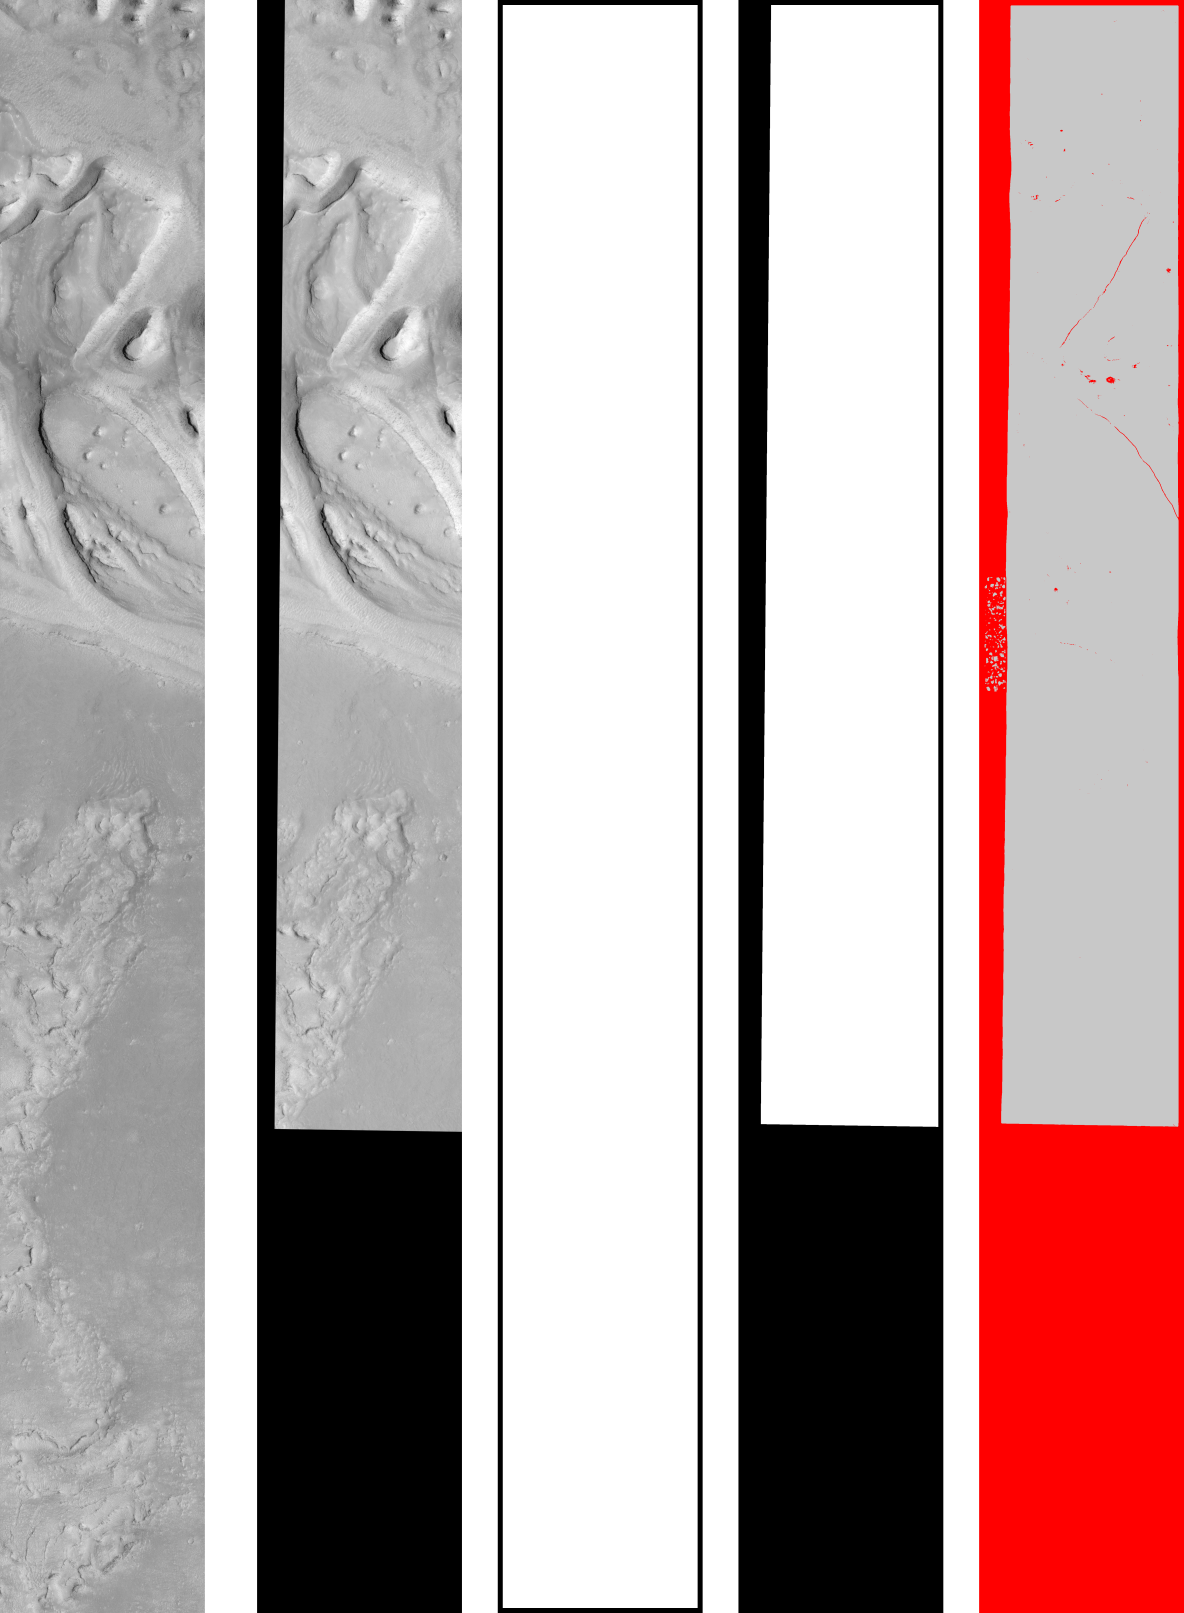
\includegraphics[width=5in]{images/p19-stereo-output.png}
\caption[P19 stereo output images]{
    \label{p19-stereo-output}
	These are the four viewable \texttt{.tif} files created by
	the \texttt{stereo} program.  The left two are the aligned
	images (\texttt{E0201461-M0100115-L.tif} and
	\texttt{E0201461-M0100115-R.tif}).  The next two images are
	the mask images (\texttt{E0201461-M0100115-lMask.tif} and
	\texttt{E0201461-M0100115-rMask.tif}), which indicate which
	pixels in the aligned images are good to use for the next
	step.  The image on the right is the Good Pixel map
	(\texttt{E0201461-M0100115-GoodPixelMap.tif}), which indicates
	the pixels in grey which were successfully matched with the
	correlator.  The red pixels were not.  Those red pixels which
	are not black in both mask images are optionally filled later
	during the hole-filling step.
    }
\end{center}
\end{figure}

% \begin{figure}
% \begin{center}
% \includegraphics[height=8in]{images/p19-goodpixel.png}
% \caption[P19 good pixel image]{
%     \label{p19-goodpixel}
% 	The Good Pixel map.
% 	Red pixels are not useful for alignment.
%     }
% \end{center}
% \end{figure}
%
% \begin{figure}
% \begin{center}
% \includegraphics[width=3in]{images/p19-aligned.png}
% \caption[P19 aligned image]{
%     \label{p19-aligned}
% 	The left and right aligned images.
%     }
% \end{center}
% \end{figure}

If those TIFF files look okay, you can probably just go on to making
a mesh or a DTM from the point cloud file
(\texttt{E0201461-M0100115-PC.tif}).  The most important file is
the Good Pixel Map (\texttt{E0201461-M0100115-GoodPixelMap.tif}).
If this file shows mostly good, gray pixels in the overlap area
(the area that is white in both the \texttt{E0201461-M0100115-lMask.tif}
and \texttt{E0201461-M0100115-rMask.tif} files), then you're probably
good to go.  If this shows bad, red pixels in the overlap area,
then you'll probabaly need to go back and tune your \texttt{stereo.default}
file.  The example data also contains a \texttt{stereo.bad} file
which has intentionally bogus values for the dimensions of the
correlation window.  You can run \texttt{stereo} with the \texttt{-s
stereo.bad} command to see what the Good Pixel Map looks like with
this.

To get an idea of the disparity information that the \texttt{stereo}
program created and then used to build the point cloud, it can be
useful to take a look at that disparity information.  The \texttt{stereo}
program records this information in several \texttt{.exr} disparity
files.

To get a look at the disparity information, you need to convert it
into a more viewable format.  Move into the directory that contains
your results, and run the \texttt{disparitydebug} program (page
\pageref{disparitydebug}) to create the the horizontal and vertical
components of the disparity (matching offsets for each pixel).

\begin{figure}[b!]
\begin{minipage}{4in}
\includegraphics[width=4in]{images/p19-disparity.png}
\end{minipage}
\hfill
\begin{minipage}{2.7in}
\caption[P19 disparity images]{
    \label{p19-disparity}
	The disparity images.  The two images on the left are the
	\texttt{E0201461-M0100115-D-H.tif} and
	\texttt{E0201461-M0100115-D-V.tif} files, which are the raw horizontal and
	vertical disparity components.  The two images on the right are the
	\texttt{E0201461-M0100115-F-H.tif} and
	\texttt{E0201461-M0100115-F-V.tif} files, which are the final
	filtered, sub-pixel disparity map with outlier removal and holes
	filled in, and is what will be used to build the point cloud.  Since
	these MOC images were acquired by rolling the spacecraft across-track,
	most of the disparity that represents topography is present in the
	horizontal disparity map.  The vertical disparity map shows disparity
	not from topography, but from spacecraft movement.
    }
\end{minipage}
\end{figure}

\begin{verbatim}
    cd results
    disparitydebug E0201461-M0100115-F.exr
\end{verbatim}

\noindent
The two output files, \texttt{E0201461-M0100115-F-H.tif} and
\texttt{E0201461-M0100115-F-V.tif} are normalized images of the
horizontal (H) and vertical (V) disparity.  `Normalized' is a key
word here.  You can see that the horizontal and vertical disparity
images in figure \ref{p19-disparity} have the same range of gray
values from white to black, but they represent significantly different
absolute amounts of disparity.  These files are useful if you want
to check the performance of the \texttt{stereo} program for any
given stereo pair.

There are actually four flavors of disparity map: the \texttt{-D.exr},
the \texttt{-R.exr}, the \texttt{-F-corrected.exr}, and \texttt{-F.exr}.
You can run \texttt{disparitydebug} on any of them, and actually taking a
look at all of them can show you the differences between the disparity maps
at the different stages of processing.

When \texttt{stereo} finishes up, it will have produced a point cloud.
At this point, the processing fans out, as many kinds of data
products can be built from the \texttt{E0201461-M0100115-PC.tif}.

One of the things that can be done is to produce a 3D mesh with
\texttt{point2mesh} (page \pageref{point2mesh}). This is not a science
product, but is just a quick visualization that can show the data
rendered in 3D. The mesh produced can be viewed with
\texttt{osgviewer} (the Open Scene Graph Viewer program, distributed
with the binary version of the Stereo Pipeline).  The
\texttt{point2mesh} program takes the point cloud file and the left
normalized image created by \texttt{stereo} as inputs.

\begin{verbatim}
    point2mesh E0201461-M0100115-PC.tif E0201461-M0100115-L.tif -l
\end{verbatim}

\noindent
This will create the file \texttt{E0201461-M0100115.ive}, openable
with \texttt{osgviewer}. When the \texttt{osgviewer} program starts,
you may want to turn off the lighting (hit the `L' key).

\begin{figure}[h]
\begin{minipage}{5in}
\includegraphics[width=5in]{images/p19-osg.png}
\end{minipage}
\hfill
\begin{minipage}{1.7in}
\caption[P19 in OSG]{
    \label{p19-osg}
	This shows the \texttt{E0201461-M0100115.ive} file displayed in
	the OSG Viewer.
    }
\end{minipage}
\end{figure}

The \texttt{point2dem} program (page \pageref{point2dem}) creates
a digital elevation model (DEM) from the Point Cloud file.

\begin{verbatim}
    point2dem E0201461-M0100115-PC.tif
\end{verbatim}

The resultant file, \texttt{E0201461-M0100115-DEM.tif}, will have
32-bit pixels, and so (much like the \texttt{E0201461-M0100115-PC.tif}
file) will not render well in typical image viewers. The resulting TIF
file is also contain georeferencing information which is useful for
working with other GIS platforms.

You can specify a coordinate system (e.g., latlon) and a reference
spheroid (i.e., calculated for the Moon or Mars). You also have the
option of creating a normalized DEM in addition to the automatically
generated non-normalized DEM. The normalized DEM again is just for
visualization and checking the quality of the product.

\begin{verbatim}
    point2dem --xyz-to-lonlat -r mars -n E0201461-M0100115-PC.tif
\end{verbatim}

\noindent
The \texttt{point2dem} program can also be used to orthoproject raw
satellite imagery onto the DEM. To do this, invoke \texttt{point2dem}
just as before, but add the \texttt{orthoimage} option and specify
the use of the left image file as the texture file to use for the
projection

\begin{verbatim}
    point2dem --xyz-to-lonlat -r mars --orthoimage E0201461-M0100115-L.tif \
      E0201461-M0100115-PC.tif
\end{verbatim}

\noindent
The \texttt{point2dem} program can be used in many different ways.
Be sure to explore all of the options.

\begin{figure}
\begin{minipage}{4in}
\includegraphics[width=4in]{images/p19-norm_ortho.png}
\end{minipage}
\hfill
\begin{minipage}{2.7in}
\caption[P19 Normalized DEM and Orthophoto]{
    \label{p19-norm_ortho}
	The image on the left is a normalized DEM (using the
	\texttt{-n} option) which which shows low terrain values
	as black and high terrain values as white (in a 0 to 255
	sense).  The image on the right is the orthographic image
	(created using the \texttt{--orthoimage} option to
	\texttt{point2dem}).
    }
\end{minipage} \end{figure}

% \begin{figure}
% \begin{center}
% \includegraphics[width=4in]{images/p19-dems.png}
% \caption[P19 dem images]{
%     \label{p19-dems}
% 	The non-normalized and normalized DEMs. Note that the
% 	non-normalized version contains floating point pixel values
% 	and will not open in most image viewing programs which
% 	expect integer pixel values between 0 and 255 (which is
% 	what the normalized version does for you).
%     }
% \end{center}
% \end{figure}
%
% \begin{figure}
% \begin{center}
% 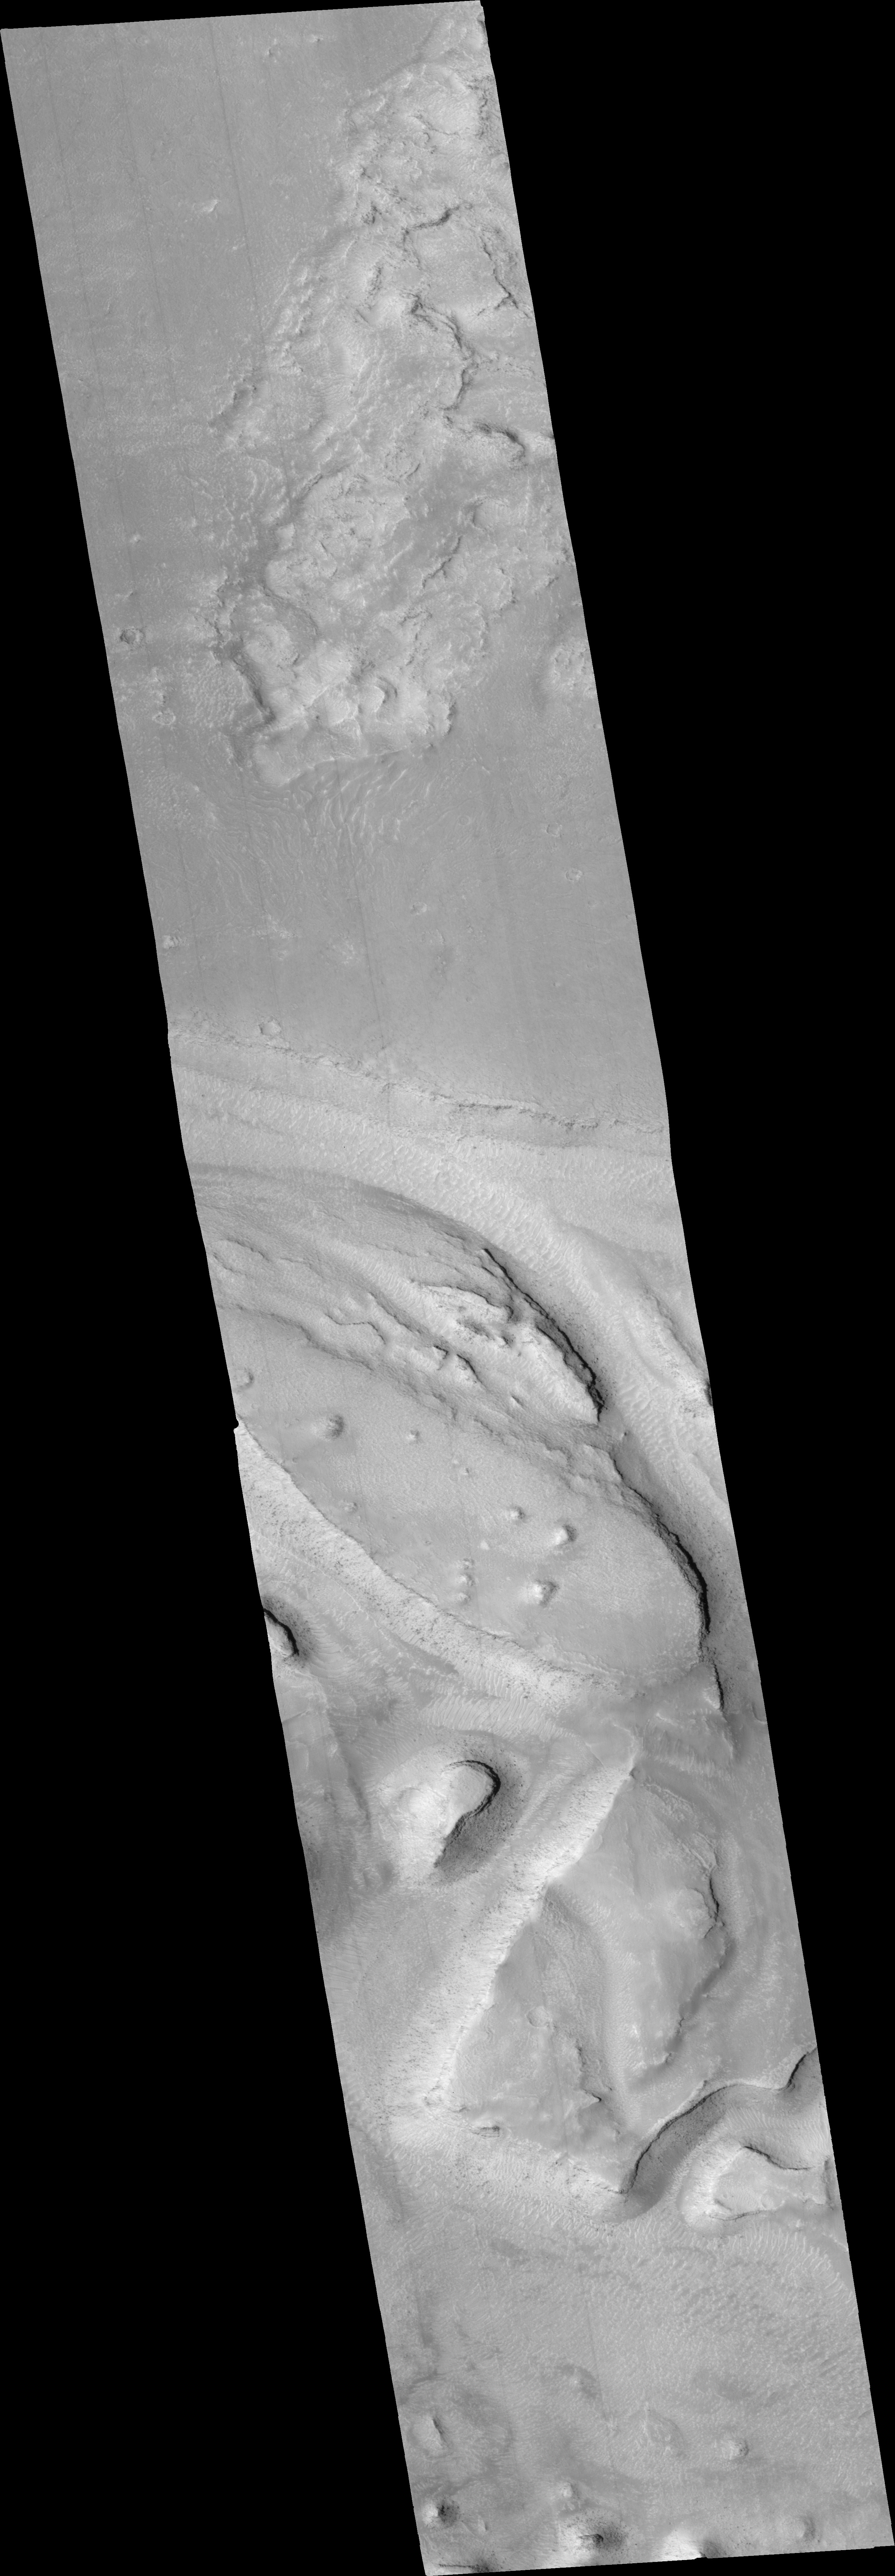
\includegraphics[width=3in]{images/p19-ortho.png}
% \caption[P19 orthophoto]{
%     \label{p19-ortho}
% 	The left image orthoprojected onto the DEM.
%     }
% \end{center}
% \end{figure}

Once you have generated a DEM file, you can use the Vision Workbench's
\texttt{colormap} and \texttt{hillshade} tools to create colorized
and/or shaded relief images from the DEM.

To create a colorized version of the DEM, you need only specify the
DEM file to use. Yet alternatively you can specific your own min and
max color ranges.

\begin{verbatim}
    colormap p19-DEM.tif -o p19-colorized.tif
\end{verbatim}

To create a hillshade of the DEM, you should specify the DEM file
to use. It is also advisable to explore the effects of altering the
elevation of the light source.

\begin{verbatim}
    hillshade p19-DEM.tif -o p19-shaded.tif -e 25
\end{verbatim}

To create a colorized version of the shaded relief file, specify
the DEM and the shaded relief file that should be used.

\begin{verbatim}
    colormap p19-DEM.tif --shaded-relief-file p19-shaded.tif -o p19-color-shaded.tif
\end{verbatim}

\begin{figure}
\begin{center}
\includegraphics[width=5in]{images/p19-colorized-shaded.png}
\caption[P19 colorized and shaded relief]{
    \label{p19-color}
	The colorized DEM, the shaded relief image, and the colorized hillshade.
    }
\end{center}
\end{figure}

The final option of the stereo processing package is
\texttt{image2qtree}.  This function was designed for use in creating
geographically referenced images in tiles such that each tile can be
viewed at ideal resolution. It can also be used to create KML files
that can be viewed in Google Earth. The program can be used on any of
the following files that you have generated:
\begin{verbatim}
    p19-DEM-normalized.tif
    p19-DRG.tif
    p19-shaded.tif
    p19-colorized.tif
    p19-shaded-colorized.tif
\end{verbatim}

Specify which image you would like to invoke \texttt{image2qtree}
on. Below makes an overlay that can be viewed in Google Mars.

\begin{verbatim}
    image2qtree p19-DEM-normalized.tif -m kml --draw-order 100
\end{verbatim}


%% \section{Preparing Selected Data}

%% There are many ways to process different kinds of image data, and
%% some will be more appropriate for operations by the Stereo Pipeline
%% than others.  While we strive to make the Stereo Pipeline extensible
%% and robust, there are a limited (but growing) set of data that we
%% have thoroughly tested.

%% This section outlines the suggested pre-processing steps to prepare
%% specific data sets for use in the Stereo Pipeline.

%% \subsection{Mars Oribiter Camera (MOC)}

%% MOC images (ending in \texttt{.imq} or \texttt{.img}) can be downloaded from
%% the PDS and only require a single ISIS command to prepare for Stereo Pipeline use:

%% \begin{verbatim}
%%     ISIS 3> mocproc from= MOCimage.imq to= MOCimage.cub Mapping= NO
%% \end{verbatim}

%% The resulting ISIS cube file (e.g. \texttt{MOCimage.cub}) is now ready
%% for processing by the \texttt{stereo} program.


%% \subsection{High Resolution Imaging Science Experiment (HiRISE)}

%% HiRISE images are more complicated.

%% At the moment, the `best' processing method is to start with HiRISE
%% \texttt{*.balance.cub} files (available only internally to the
%% HiRISE team) and run them through the USGS's \texttt{hinoproj.pl}
%% script.  This results in \texttt{noproj}ed and de-jittered cube
%% files that can be run.

%% In the future (who knows when), the HiRISE team will directly produce
%% \texttt{noproj}ed images (dejittered through a different, improved,
%% algorithm) which will be available in the \texttt{extras/} directory
%% of the HiRISE PDS Volume.  And those images will probably be directly
%% usable by the Stereo Pipeline.

%% \emph{As you can tell, I'm still in the process of tracking all of this down. -RAB}

\chapter{Programs}

This chapter covers the various user-programs that are a part of
the Ames Stereo Pipeline.

\section{stereo}

The \texttt{stereo} program is the primary workhorse of the Ames
Stereo Pipeline.  It is the program that takes a pair of images which
overlap and creates an output point cloud which can then be fed to the
\texttt{point2mesh} or \texttt{point2dem} programs.

\emph{Way more needs to go in here ...}

\subsection{stereo.default file}

The \texttt{stereo.default} file contains configuration parameters
which the \texttt{stereo} program uses to process the images.  Below
we will walk through the contents of the \texttt{stereo.default.example}
file distributed with the Ames Stereo Pipeline and discuss all of
the various parameters.

The parameters which begin with `\texttt{DO\_}' are true/false options,
when set to `1' they are `on' or `true,' and if set to `0' they are
`off' or `false.'

The parameters below also have their default values listed after
the parameter name.

\subsubsection*{Preprocessing}

\begin{description}
\item[DO\_INTERESTPOINT\_ALIGNMENT 1] \hfill \\
When \texttt{DO\_INTERESTPOINT\_ALIGNMENT} is on (or set to 1), ... \emph{MJB: describe}

\item[DO\_EPIPOLAR\_ALIGNMENT 0] \hfill \\
By default this is off.  When on ... \emph{MJB: describe}

\item[INTERESTPOINT\_ALIGNMENT\_SUBSAMPLING 1] \hfill \\
This option allows you to change the density of interest points
that stereo will find, correlate, and result in the final point
cloud.  When this is set to 1, there is no subsampling, the
\texttt{stereo} program will do its best to find as many interest
points within the imagery as it can.  When this is set to 2, the
program will ignore every other interest point that it finds, and
will only process the reduced set.  This parameter can be set to
any positive integer.  When this parameter is turned up, the resulting
point cloud will have less effective resolution.

\item[DO\_SLOG 1 and DO\_LOG 0] \hfill \\
These two items are related, only one can be set to `on', if both
are `on' the program will default to doing only SLOG.  \emph{MJB: explain the difference}

\item[SLOG\_KERNEL\_WIDTH 1.5] \hfill \\
When \texttt{DO\_SLOG} is `on,' this option sets the diameter of
the convolution kernel. \emph{MJB: describe}

\end{description}

\subsubsection*{Correlation}
\subsubsection*{Filtering}
\subsubsection*{Dot Cloud}

\section{disparitydebug}
\section{results}
\section{point2mesh}
\section{point2dem}
\section{orthoproject}

\chapter{Bundle Adjustment}

Bundle adjustment is the process of simultaneously adjusting the
properties of multiple cameras and the 3D locations of the objects
they see, to minimize the error between the estimated forward
projection of the 3D objects and their measured location in the captured
images. 

\begin{figure}[htp]
  \begin{center}
  \includegraphics[trim=20mm 20mm 20mm 15mm,clip,width=6in]{images/ba_feature_observation.pdf}
  \end{center}
  \caption{ A feature observation in Bundle Adjustment. \cite{moore09} }
  \label{fig:ba_feature}
\end{figure}

This has application as an optional step between the capture
of images and the creation of DEMs. There is always an amount of error
with the recorded position and orientation of cameras and Bundle
Adjustment can be used to refine these measurements. This will allow
DEMs from multiple cameras to align better with one another. Bundle
Adjustment can also take advantage of Ground Control Points (GCPs),
which are accurately measured 3D locations on the surface of the DEM. GCPs
can be used to improve the alignment of the DEMs or align the new DEM
to a past data product. Finally, even though Bundle Adjustment
calculates the location of the 3D objects it views, only the final
properties of cameras are recorded in the Ames Stereo Pipeline. Those
properties are loaded into \texttt{stereo} which will then use it's own
method for triangulation.

\subsection{A deeper understanding}

Bundle Adjustment in Ames Stereo Pipeline revolves around the
Levenberg-Marquardt Algorithm (LMA) which is a method for minimizing a
function. In the case of Bundle Adjustment, the error $\epsilon$ is
the pixel difference between an objects location in an image,
$[u_{f},v_{f}]$, and it's forward projection through the camera,
$[\tilde{u}_{f},\tilde{v}_{f}]$. The goal is to solve for an update to
the parameters of the cameras and point positions, apply them, and
then repeat until the update supplied by LMA goes to zero. The
equation for LMA is below:

\begin{equation}
\mbox{\boldmath$\delta$} = \frac{\mbox{\boldmath$J^T\epsilon$}}{\bf{J^TJ}+\lambda\bf{I}}
\label{eqn: Levenberg-Marquardt Algorithm}
\end{equation}

LMA is a hybrid of two minimization techniques, gauss-newton and
gradient decent. Where the control between these two methods is the
parameter $\lambda$ which will change in value during the process of
Bundle Adjustment. A high value of $\lambda$ forces LMA to act like
gradient decent, and is what will happen at the beginning of bundle
adjustment when the camera parameters are far away from their final
solution. A low value of $\lambda$ drives LMA into the gauss-newton
method; at which it will take small steps in updating the camera
values. When Bundle Adjustment is almost finished and is close to the
solution, it will lower $\lambda$.

Since Bundle Adjustment is an iterative method, it would be happy to
keep processing new updates to camera parameters all day. To avoid
this, there are several shut-off conditions. The first is when the
update {\boldmath$\delta$} becomes insignificantly small. The second
is when the error measurement, {\boldmath$\epsilon$}, becomes
insignificantly small. Both of these conditions' thresholds are
defined within the bundle adjuster's code and is not allowed for the
user to change. The final shut off condition is when the number of
iterations becomes too large. It is important to understand that when
this shut off condition happens, bundle adjustment has not finished
refining the parameters of the cameras but they are a step closer to
the solution. The maximum number of iterations is changeable by the
user so they can decide how much time they're will to dedicate to the
correction of the data. The number of iterations Bundle Adjustment
takes to converge on the solution can be anywhere between 20
iterations to several hundred.

If you are interested in more information on the math of Bundle
Adjustment and the arrangement of the problem, we recommend reading
Appendix 6 in the {\em Multiple View Geometry} \cite{hartley04}.
For more information on why LMA is used instead of the many other
optimization algorithms, try reading {\em Bundle Adjustment – A Modern
Synthesis} \cite{triggs00}.

\section{ISIS Adjust}

The \texttt{isis\_adjust} program is an application designed to
perform bundle adjustment on the cameras supported by USGS's
ISIS3. \texttt{isis\_adjust} is special in that it does not
discriminate based on camera type. It can perform bundle adjustment on
line-scan imagers (such as MOC and Apollo's Panoramic Camera) just as
well as it can on traditional frame cameras (such as Apollo Metric
Camera). Theoretically it should also work fine with push-frame
imagers (i.e. video), though this is untested.

\texttt{isis\_adjust} works by first converting all pixel measurements
in an images to measurements defined on the ideal focal
plane using millimeters and the ephemeris time (ET). The ET is the
absolute second at which that pixel measurement was recorded on the camera. 
For a frame camera, the ET won't change for the for
any of the measurements on the image. For anything more exotic, it is
a different story. On a MOC image between the top and bottom line;
about 5 seconds could have passed.

\begin{wrapfigure}{r}{0.3\textwidth}
\vspace{-30pt}
\begin{center}
  \definecolor{lgray}{gray}{0.95}
  \fcolorbox{black}{lgray}{\begin{minipage}{0.29\textwidth} 

      \emph{Note from Author:} \\ Currently \texttt{isis\_adjust}
      lacks a proper way to support arbitrary defined correction
      functions. For the time being, \texttt{isis\_adjust} has been
      hard-coded to perform only zero order corrections (i.e. scalar
      offsets). (03/11/09)

  \end{minipage}}
\end{center}
\vspace{-30pt}
\end{wrapfigure}

When \texttt{isis\_adjust} calculates the partial derivatives of the
forward projection of a point, it will use an ideal pinhole camera
model. The properties of the ideal pinhole camera are defined as
properties of the subject camera at the specificed ET for the current
measure plus the correction function $f(t)$ that \texttt{isis\_adjust} is
solving for. $f(t)$ can be almost any function of ET, the only limit is the
number parameters in the equations. Some initial work hints that
anything greater than a $2^{nd}$ order polynomial becomes an ill-posed
problem.

\subsection{Options}

\begin{verbatim}
--cnet, -c [control network file]
\end{verbatim}

\emph{Optional.} Feeding this option will force ISIS Adjust to use an
already built control network. If not fed, ISIS Adjust will look for
match files in current operating directory with names similar to the
input images to build it's control network from. If
\texttt{isis\_adjust} creates it's own control network file, it will
save it as \verb=isis_adjust.cnet=.

\begin{verbatim}
--lambda, -l [value]
\end{verbatim}

\emph{Optional.} This set the starting value for $\lambda$. Bundle
Adjustment will naturally select a value for $\lambda$ it thinks is
best for the starting error, but this argument can be used to override
that. \emph{It's not recommended to change the starting value of
  $\lambda$ except for experienced users.}

\begin{verbatim}
--position-sigma [default = 100]
\end{verbatim}

Sets the sigma \emph{(uncertainty)} of the spacecraft position in
meters.

\begin{verbatim}
--pose-sigma [default = 0.1]
\end{verbatim}

Sets the sigma \emph{(uncertainty)} of the spacecraft pose in radians.

\begin{verbatim}
--gcp-sigma [default = 100]
\end{verbatim}

Sets the sigma \emph{(uncertainty)} of the ground control points in
meters.

\begin{verbatim}
--run-match, -m
\end{verbatim}

\emph{Optional.} If match files don't already exist, create them using a
call to \texttt{IPmatch}.

\begin{verbatim}
--match-debug-images, -d
\end{verbatim}

\emph{Optional.} If a call to \texttt{ipmatch} is being called, this option
also allows for the creation of debugging images that show the matches
between the input images.

\begin{verbatim}
--min-matches [default = 5]
\end{verbatim}

When producing a control network, this sets the minimum required
interest point matches between images for them to be included. If a
match file fails to find this many of matches, it probably means these
were poor matches and the images don't really overlap.

\begin{verbatim}
--max-iterations [default = 25]
\end{verbatim}

Sets the maximum number of iterations to be done by Bundle Adjustment.

\begin{verbatim}
--report-level, -r [default = 10]
\end{verbatim}

Sets the report level for the final report on the bundle adjustment
which can be found in \verb=rmax_adjust.report=. Report levels are defined in
BundleAdjustReport.h in Vision Workbench.

\begin{verbatim}
--nonsparse, -n
\end{verbatim}

\emph{Optional.} Switches the Bundle Adjustment code to use non-sparse
matrices in it's math. \emph{This will cause it to run significantly slower
and is only used as a check of the programmer's sparse matrix code.}

\begin{verbatim}
--write-isis-cnet-also
\end{verbatim}

\emph{Optional.} Write an ISIS PVL style control network file in
\verb=isis_adjust.net=. The output file is very large compared to the
binary output, \verb=isis_adjust.cnet=, and is human readable. This
alternative's importance is that it can be used with ISIS3's
\texttt{Qnet}.

\subsection{Examples of Use}

%\begin{wrapfigure}{r}{2.5in}
%\begin{center}
%  \definecolor{lgray}{gray}{0.95}
%  \fcolorbox{black}{lgray}{\begin{minipage}{2.2in} Hey! Hi we at IRG
%      actually use SURF! Blag sg f d fgds dfsgd srd sssf ds dfs fsdf
%      sd fdsrds rdsr drdf dgsrr ge gerges s i srges ge
%  \end{minipage}}
%\end{center}
%\end{wrapfigure}

What follows is an example of using two Mars Orbital Camera (MOC)
images of the south Cydonia region with \texttt{isis\_adjust}. We'll
be using images M10/00254 and R09/01059. These images are available
at Malin Space Science System's website
[\emph{http://www.msss.com/moc\_gallery/}] and at NASA's Planetary
Data System [\emph{http://pds.jpl.nasa.gov/index.shtml}]; be sure to
download the IMQ or IMG format. For reference, the following ISIS commands
are how to convert the MOC images to ISIS cubes.

\begin{verbatim}
        moc2isis from=m1000254.im? to=m1000254.lev0.cub
        moc2isis from=r0901059.im? to=r0901059.lev0.cub

        spiceinit from=m1000254.lev0.cub
        spiceinit from=r0901059.lev0.cub

        moccal from=m1000254.lev0.cub to=m1000254.cub
        moccal from=r0901059.lev0.cub to=r0901059.cub

        rm *.imq *.lev0.cub
\end{verbatim}

At this point a match file needs to be created that connects our to
cube files. Vision Workbench doesn't except cube files. So before
trying to match them; they'll have to be converted to a standard image
format.

\begin{verbatim}
        isis2std from=m1000254.cub to=m1000254.png format=PNG
        isis2std from=r0901059.cub to=r0901059.png format=PNG
\end{verbatim}

Here is how to process those newly created PNG files for interest points using the tools available in Vision Workbench.

\begin{verbatim}
        ipfind  m1000254.png r0901059.png
        ipmatch m1000254.png r0901059.png -d -r homography
\end{verbatim}

\definecolor{lgray}{gray}{0.95}
\begin{center}
\fcolorbox{black}{lgray}{ \begin{minipage}{5.5in} 

    \emph{Note from Author:} \\ Within IRG it has become apparent that
    using the interest point tools available from Vision Workbench
    does not produces enough matches to continue with Bundle
    Adjustment. The alternative is to use an outside method such as
    SURF \cite{surf09}. The trick is modifing an outside method's
    source code to export a Vision Workbench style match file. This
    can be difficult. Fortunately the patches to do this trick to the
    SURF code is available in the Appendix.  \\ \\ For this example it
    is okay to use the results from \texttt{ipfind} and
    \texttt{ipmatch}. Expect to find approximately 46 matched
    points. Your results will be slightly different due to the random
    nature of RANSAC.
\end{minipage}}
\end{center}

Finally, it is time to start Bundle Adjustment. There are many options
that can be done here. Below shows the options required to create
visualization data for \texttt{bundlevis} \emph{(This is covered in
  detail in the next section)}, setting the maximium iterations to
100, and finally the option to create a detailed report file of
\texttt{isis\_adjust}'s results.

\begin{verbatim}
        isis_adjust *.cub -s --max 100 -r 50
\end{verbatim}

The command window should spurt forth a lot of text and the directory
containing this project should suddenly have a lot more files. Don't
panic! This is perfectly normal! Looking through the output in the
terminal or alternatively in the output report file,
\verb=isis_adjust.report=, the problem should have convereged in 35
iterations. The error barely changed, this can be attributed Mars
Global Surveyor's relative positioning between images being very good. 

Producing DEMs using the newly created corrections is the same as
covered in Chapter 3. There is one fine difference in that
\texttt{stereo} needs to know of the existence of the correction
files, \verb=m1000254.isis_adjust= and
\verb=r0901059.isis_adjust=. Here is how that is done:

\begin{verbatim}
        stereo m1000254.cub r0901059.cub m1000254.isis_adjust
               r0901059.isis_adjust MOC_RESULTS/M1000254_R0901059
\end{verbatim}

\texttt{stereo} is excepting the correction files in the place where it would optionally accept a camera model file. It decides what to do with the input based on the file extension, in this case it is \verb=.isis_adjust=.

\section{Visualizing Bundle Adjustment with BundleVis}

Purpose, Examples, Supported Cameras, and File Types

\begin{figure}[htp]
  \begin{center}
  \includegraphics[width=6in]{images/bundlevis_apollo.png}
  \end{center}
  \caption{ A screenshot of bundle adjustment of Apollo 15's Orbit 33. }
  \label{fig:bundlevis}
\end{figure}

\begin{thebibliography}{1}

\bibitem{hartley04} Hartley, R.I. and Zisserman, A. ``Multiple View Geometry in Computer Vision,''
  Cambridge University Press. 2004. pp 597-627.
\bibitem{moore09} Moore, Wright, Schinstock, and Lewis. ``Comparison of Bundle Adjustment Formulations,''
  presented at ASPRS Annual Conf., Baltimore, Maryland, 2009.
\bibitem{triggs00} Triggs, McLauchlan, Hartley, and Fitzgibbon. ``Bundle Adjustment - A Modern Synthesis,''
  Lecture Notes in Computer Science. Vol. 1883, 298. January 2000
\bibitem{surf09} Bay, Gool, and Tuytelaars. (2009, Mar.). ``SURF: Speeded Up Robust Features'' [Online]. Available: \verb!http://www.vision.ee.ethz.ch/~surf/download.html!

\end{thebibliography}

\appendix
\chapter{Modifying SURF to output VW match files}

What follows is the output of \texttt{diff} between the original SURF
v1.0.9 code and the modified code to write a Vision Workbench style
match file. This Appendix only applies to Linux and potentially
Windows users. SURF is currently unavailable for Mac OSX.

\section{Patch to match.cpp}

\begin{verbatim}
--- orginal_code/SURF-V1.0.9/match.cpp	2006-12-20 03:28:30.000000000 -0600
+++ match.cpp	2009-03-11 13:26:07.000000000 -0500
@@ -31,7 +31,7 @@
  */
 
 #include <vector>
-#include <string>
+#include <string.h>
 #include <iostream>
 #include <fstream>
 #include <cmath>
@@ -39,12 +39,10 @@
 #include "ipoint.h"
 
 // Define to compile with PGM output
-#define GRAPHICS
+//#define GRAPHICS
 
-#ifdef GRAPHICS
 #include "image.h"
 #include "imload.h"
-#endif
 
 using namespace std;
 using namespace surf;
@@ -69,6 +67,7 @@
 	int match = -1;
 
 	for (unsigned i = 0; i < ipts.size(); i++) {
+
 		// Take advantage of Laplacian to speed up matching
 		if (ipts[i].laplace != ip1.laplace)
 			continue;
@@ -90,6 +89,30 @@
 	return -1;
 }
 
+// Writes the interestpoint match for later reading
+inline void write_ip_record(std::ofstream &f, Ipoint const& p){
+  float buffer_f = (float)p.x;
+  f.write((char*)&(buffer_f), sizeof(float));       //x
+  buffer_f = (float)p.y;
+  f.write((char*)&(buffer_f), sizeof(float));       //y
+  int buffer_i = (int)p.x;
+  f.write((char*)&(buffer_i),   sizeof(int));         //ix
+  buffer_i = (int)p.y;
+  f.write((char*)&(buffer_i),   sizeof(int));         //iy
+  buffer_f = (float)p.ori;
+  f.write((char*)&(buffer_f), sizeof(float));     //ori
+  buffer_f = (float)p.scale;
+  f.write((char*)&(buffer_f), sizeof(float));     //scale
+  buffer_f = (float)p.strength;
+  f.write((char*)&(buffer_f),sizeof(float)); //interest
+  bool buffer_b = false;
+  f.write((char*)&(buffer_b),sizeof(bool));  //polarity
+  f.write((char*)&(buffer_i),sizeof(unsigned)); // octave
+  f.write((char*)&(buffer_i),sizeof(unsigned)); // scale_lvl
+  buffer_i = 0;
+  f.write((char*)&(buffer_i),     sizeof(int));         //size of descriptor... nothing...                                                                                                
+}  
+
 // Find all possible matches between two images
 vector< int > findMatches(const vector< Ipoint >& ipts1, const vector< Ipoint >& ipts2) {
 	vector< int > matches(ipts1.size());
@@ -98,9 +121,7 @@
 		int match = findMatch(ipts1[i], ipts2);
 		matches[i] = match;
 		if (match != -1) {
-			cout << " Matched feature " << i << " in image 1 with feature "
-				<< match << " in image 2." << endl;
-			c++;
+		  c++;
 		}
 	}
 	cout << " --> Matched " << c << " features of " << ipts1.size() << " in image 1." << endl;
@@ -127,10 +148,10 @@
 	// Load the interest points in Mikolajczyk's format
 	for (unsigned n = 0; n < count; n++) {
 		// circular regions with diameter 5 x scale
-		float x, y, a, b, c;
+	  float x, y, a, b, c, ori;
 
 		// Read in region data, though not needed for actual matching
-		ipfile >> x >> y >> a >> b >> c;
+	  ipfile >> x >> y >> a >> b >> c >> ori;
 
 		float det = sqrt((a-c)*(a-c) + 4.0*b*b);
 		float e1 = 0.5*(a+c + det);
@@ -142,6 +163,7 @@
 		ipts[n].x = x;
 		ipts[n].y = y;
 		ipts[n].scale = sc/2.5;
+		ipts[n].ori = ori;
 
 		// Read in Laplacian
 		ipfile >> ipts[n].laplace;
@@ -159,7 +181,7 @@
             (y1 >= im->getHeight() && y2 >= im->getHeight()))
 		return;
 
-	bool steep = std::abs(y2 - y1) > std::abs(x2 - x1);
+	bool steep = abs(y2 - y1) > abs(x2 - x1);
 	if (steep) {
 		int t;
 		t = x1;
@@ -182,7 +204,7 @@
 	}
 
 	int deltax = x2 - x1;
-	int deltay = std::abs(y2 - y1);
+	int deltay = abs(y2 - y1);
 
 	int error = 0;
 	int y = y1;
@@ -215,12 +237,14 @@
 
 int main(int argc, char **argv) {
 	Image *im1, *im2;
-#ifdef GRAPHICS
+
 	ImLoad ImageLoader;
 	vector< Ipoint > ipts1, ipts2;
 	bool drawc = false;
-#endif
+
 	char ofname[100];
+	string matchname;
+	matchname.clear();
 
 	im1 = im2 = NULL;
 	ofname[0] = 0;
@@ -232,7 +256,6 @@
 			loadIpoints(argv[++arg], ipts1);
 		if (! strcmp(argv[arg], "-k2"))
 			loadIpoints(argv[++arg], ipts2);
-#ifdef GRAPHICS
 		if (! strcmp(argv[arg], "-im1"))
 			im1 = ImageLoader.readImage(argv[++arg]); 
 		if (! strcmp(argv[arg], "-im2"))
@@ -241,12 +264,13 @@
 			strcpy(ofname, argv[++arg]);
 		if (! strcmp(argv[arg], "-c"))
 			drawc = true;
-#endif
+		if (! strcmp(argv[arg], "-m"))
+		  matchname = argv[++arg];
 	}
 
 	if (ipts1.size() == 0 || ipts2.size() == 0) {
 		cout << "Usage:" << endl;
-		cout << " match -k1 out1.surf -k2 out2.surf -im1 img1.pgm -im2 img2.pgm -o out.pgm" << endl << endl;
+		cout << " match -k1 out1.surf -k2 out2.surf -im1 img1.pgm -im2 img2.pgm -o out.pgm -m output.match" << endl << endl;
 		cout << "For each feature in first descriptor file, find best in second according to "
 			<< "nearest neighbor ratio strategy. Display matches in out.pgm, generated "
 			<< "from img1.pgm and img2.pgm. Use -c to draw crosses at interest points." << endl;
@@ -255,7 +279,33 @@
 
 	vector< int > matches = findMatches(ipts1, ipts2);
 
-#ifdef GRAPHICS
+	// Determining if to save a match file
+        if (matchname.size()) {
+          int count = 0;
+          for (unsigned i = 0; i < matches.size(); ++i){
+            if (matches[i] != -1)
+              ++count;
+          }
+          if (count > 0 ) {
+            std::ofstream outputFile(matchname.c_str(), std::ios::out);
+            outputFile.write((char*)&count, sizeof(int));
+            outputFile.write((char*)&count, sizeof(int));
+            //Writing left side..
+            for (unsigned i = 0; i < matches.size(); ++i){ 
+              if (matches[i] != -1) {
+                write_ip_record(outputFile,ipts1[i]);
+              } 
+            }
+            //Writing right side..
+            for (unsigned i = 0; i < matches.size(); ++i){
+              if (matches[i] != -1) {
+                write_ip_record(outputFile,ipts2[matches[i]]);
+              }  
+            } 
+          } 
+        } 
+
+
 	if (im1 != NULL && im2 != NULL && ofname[0] != 0) {
 		Image res(max(im1->getWidth(), im2->getWidth()), im1->getHeight() + im2->getHeight());
 		for (int x = 0; x < im1->getWidth(); x++)
@@ -283,7 +333,6 @@
 
 		ImageLoader.saveImage(ofname, &res);
 	}
-#endif
 	
 	return 0;
 }

\end{verbatim}

\section{How to apply and compile}

First move to the directory containing your copy of the SURF v1.0.9
code. Then copy the contents of the section above into a newly created
file called, \verb=match_cpp.diff=. Alternatively a copy of
\verb=match_cpp.diff= is included in the Appendix directory that is
inside the directory containing this documentation. At this point you
are ready to start running the following commands.

\begin{verbatim}
        patch < match_cpp.diff
        make match.ln
\end{verbatim}

\definecolor{lgray}{gray}{0.95}
\begin{center}
\fcolorbox{black}{lgray}{ \begin{minipage}{5.5in} 

    \emph{Note:} \\ If you are unfortunate enough to run into an error
    such as \textit{g++-4.0.2: Command not found}, don't worry. Edit
    \texttt{Makefile} at line 10 and 11 to refer to \texttt{g++}
    instead of \texttt{g++-4.0.2}. \\ \\ Also since you've incurred
    that error, you'll probably need to add an include to
    \texttt{<stdlib.h>} in \texttt{imload.cpp} in the same
    directory. This all stems from differences in using a newer
    version of g++.
\end{minipage}}
\end{center}

\section{Example of using SURF}

For this example it is assumed you have a directory containing two
images named \verb=m1000254.png= and \verb=r0901059.png= like in the
example found in Section 5.3.1.

SURF code only works with images in the grayscale format PGM. A free
Linux utility to convert the images is \texttt{mogrify}. That utility
is a part of the package \texttt{imagemagick} and is likely to be
available in most package managers.

Below is the commands to take an input of PNG files, process them with
SURF, and then finally create a match file which can be used by the
likes of \texttt{isis\_adjust}.

\begin{verbatim}
        mogrify -format pgm m1000254.png r0901059.png
        surf.ln -i m1000254.pgm -o m1000254.surf
        surf.ln -i r0901059.pgm -o r0901059.surf
        match.ln -k1 m1000254.surf -k2 r0901059.surf
                 -im1 m1000254.pgm -im2 r0901059.pgm
                 -o out.pgm -m m1000254__r0901059.match
        rm m1000254.pgm r0901059.pgm *.surf
\end{verbatim}

\begin{center}
\fcolorbox{black}{lgray}{ \begin{minipage}{5.5in} 

    It is important to note that though SURF is very good at
    performing matches it does not perform a step of RANSAC with it's
    output. There may be a couple of outliers.
\end{minipage}}
\end{center}


\chapter{Python Batch Processing}

Below is a Python script to process a large number of Apollo Metric
Camera pairs. This is meant only to serve as an example and it can be
modifed to run other commands.

\begin{verbatim}
#!/usr/bin/python

import glob;
import os;
import subprocess;

num_cores = 4;
joblist = [];
output_dir = "stereo";

def add_job( job ):
    if (len(joblist) >= num_cores):
        joblist[0].wait();
        joblist.pop(0);
    print job;
    joblist.append(subprocess.Popen(job,shell=True))
    return;

def run_cmd( left_file, right_file ):
    h_l = left_file.split(".");
    h_r = right_file.split(".");

    cmd = "stereo "+left_file+" "+right_file+" "+h_l[0]+".isis_adjust "+h_r[0]+".isis_adjust "+output_dir+"/"+h_l[0]+"__"+h_r[0]+" --threads 1"
    add_job(cmd);


files = glob.glob("*.cub");
files = sorted(files);
for left in range(0, len(files)):

    #determing how forward to look
    range_right = left + 2;
    if ( range_right > len(files) ):
        range_right = len(files);

    for right in range(left+1, range_right):
        run_cmd( files[left], files[right] );

for j in joblist:
    j.wait();

print "Done processing stereo pairs"

\end{verbatim}

\end{document}
